\chapter{Deep Learning and NLP: Distributed Representations and Language Modelling}\label{chapter:deepnlp}
Most, of the current Deep Learning research in NLP is focused on representation learning. By that, we mean that we represent our word, phrase or a sentence as a series of numerical values or a vector in a given vector subspace, which somehow captures the representation. This is an extensive area of research and the roots are based on the concept of Language Modeling.  
\section{Language Modelling}
A language model is a probabilistic model that assigns probabilities to any sequence of words. Such as: 
\begin{center}
\textit{p(${w}_{1}$, ... , ${w}_{T}$)}
\end{center}
Language modeling is the task of learning a language model that assigns high probabilities to well formed sentences. We take into consideration: nth order Markov assumption, where we assume that the ${i}^{th}$ word was generated based only on the n-1 previous words. It plays a crucial role in speech recognition and machine translation systems. 

\begin{figure}[ht!]
  \centering
  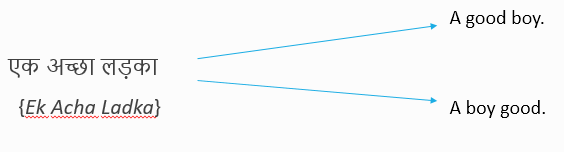
\includegraphics[height=25mm,  width=80mm]{figures/4_languagemodellingex.png}
  \caption[Language Modeling Example]{Translation of a Hindi language Sentence to English language }
  \label{languagemodellingex}
\end{figure}

Consider the example in \autoref{languagemodellingex}. We can see that the Hindi language sentence can be translated in two different ways. First, \textit{A good boy} and second,  \textit{A boy good}. What a good language model will tell us that the first one is the correct and more generally used form of the sentence. This is the power and importance of language modeling and is in the heart of all the current unsupervised natural language processing machine learning algorithmic tasks.

\subsection{Language Modelling using Ngrams}

An N-gram is defined as a sequence of n-words. For example:

\textbf{unigrams} (n=1): “is’’, ‘‘a’’, ‘‘sequence’’, etc.

\textbf{bigrams} (n=2): [‘‘is’’, ‘‘a’’ ], [‘‘a’’, ‘‘sequence’’ ], etc.

\textbf{trigrams} (n=3): [‘‘is’’, ‘‘a’’, ‘‘sequence’’], [ ‘‘a’’, ‘‘sequence’’, ‘‘of’’], etc.

The \textbf{n-gram models} estimate the conditional from n-grams counts.
\begin{center}
\begin{equation}
P({w}_{t} | {w}_{t - (n-1)}  , ...... , {w}_{t-1}) = \frac{count({w}_{t - (n-1)}  , ...... , {w}_{t-1}, {w}_{t} )}{count({w}_{t - (n-1)}  , ...... , {w}_{t-1})}
\end{equation}
\end{center}
The counts are obtained from a training corpus (a data-set of word text)

We want the value of \textbf{n} to be large, for the model to be realistic. But, for large values of \textbf{n}, it is likely that a given n-gram will not have been observed in the training corpora. Smoothing helps but only partially!

\subsection{Word Representations}
In context of current problem, we use usupervised deep learning techniques, to learn a word representation C(w) which is a continuous vector and is both syntactically and semantically similar. 
More precisely, we learn a continuous representation of words and would like the distance $||C(w)-C(w’)||$ to reflect meaningful similarity between words \textbf{w} and \textbf{w’}.

Chiefly, we explore the following word representations: Word2Vec, Polyglot, GloVe and their concatenated combinations along with Bag of Words representation and compare their results for the task of sentiment analysis.
\newline

A traditional view of the word representation is the \textbf{bag of words} or \textbf{one-hot vector} representation for the word. In this model, a text (such as a sentence or a document) is represented as the bag (multi-set) of its words, disregarding grammar and even word order but keeping multiplicity. Example: Suppose we have two documents D1 and D2
\newline

\textbf{D1:} \textit{John likes to watch movies. Mary likes movies too.}
\newline

\textbf{D2:} \textit{John also likes to watch football games.}
\newline

\textbf{Vocabulary \{Word : Index\}}
\newline

{   "John": 1,    "likes": 2,     "to": 3,     "watch": 4,     "movies": 5,     "also": 6,     "football": 7,     "games": 8,     "Mary": 9,     "too": 10 }
\newline

There are 10 distinct words and using the indexes of the Vocabulary , each document is represented by a 10-entry vector:
\newline

\textbf{[1, 2, 1, 1, 2, 0, 0, 0, 1, 1]}

\textbf{[1, 1, 1, 1, 0, 1, 1, 1, 0, 0]}
\newline 

There is a concern that in this representation, the more frequent words are weighted more than less frequent words. So, to normalize the weights across documents another representation called TF-IDF (Term Frequency - Inverse Document Frequency) is introduced.The main cause of concern with BOW and TF-IDF representation is they don't make the use of contextuality of words in the corpus. Thus, there is no way of distinguishing the order of the words correctly through this vector representation. A more recent view on this is taken through neural language modeling and it brings forward a new concept known as \textbf{Word Embeddings}. On the contrary to the one-hot representation, they build on a concept of \textbf{Distributed Representations}.
\newline

Originally, word embeddings were introduced by Bengio et al., ~\parencite{bengio1} ~\parencite{bengio2} a few years before the discussed 2006 deep learning renewal, at a time when neural networks were not that popular. Although, the idea of distributed representations for symbols is much more older, as proposed by Hinton et. al.~\parencite{hinton1}  

A \textbf{word embedding} \textit{W} : words $\Rightarrow {R}^{n}$ is a paramaterized function mapping words in some language to high-dimensional vectors (150 - 600 dimensions). For example, we might find:

W(‘parrot") = (0.3, -0.5, 0.7, ...)

W(‘‘carrot") = (0.0, 0.6, -0.1, ...)
\newline

Typically, the function is a lookup table, parameterized by a matrix, $\theta$, with a row for each word: ${W}_{\theta}({w}_{n})={\theta}_{n}$. W is first initialized randomly for each word. When we train the word vector matrix, it learns to have meaningful vectors in order to perform some task.
\newline

For example, we can train a neural network to predict whether a 5-GRAM (sequence of five words) is correct or 'valid'.  We can start with 5-grams from Wikipedia corpus (Ex.. “plane is going to fly”) and then corrupt half of them by switching a word with a random word (eg. “plane is drunk to fly”), thus, almost certainly making our corrupted 5-gram absolute nonsense.The neural network we train will feed each word in the 5-gram through W to get a vector representing it as intermediate output and feed those intermediate results into another layer say 'L' which tries to predict if the 5-gram is ‘valid’ or ‘corrupt.’~\parencite{bottou} We would obtain something like:
\newline

L(W("plane"), W(‘‘is"), W(‘‘going"), W(‘‘to"), W(‘‘fly"))=1
\newline

L(W("plane"), W(‘‘is"), W(‘‘drunk"), W(‘‘to"), W(‘‘fly"))=0
\newline

In order to predict these values accurately, the network needs to learn good parameters for both W and L. This is accomplished through back-propagation, which we have already covered earlier.
\newline

An interesting side effect which is observed, with these word vectors, is when trained on a very large corpus like Google News, the vectors for days like Tuesday and Wednesday fall close to one another in high dimensional space.  It's not just limited to days, but also gender, where the same gender words fall in a certain cluster group and difference between the tow gender entities is captured across relations. For Example:
\begin{center}
\textit{v("king") - v("queen") = v("man") - v("woman")}
\end{center}
These are interesting relationships which are somehow giving the sense that they capture the semantic similarity in vector space. Thus, with such results, the entire field of Deep Learning and NLP looks really fascinating. Next, we will discuss some of the recent methods, which have contributed strongly to this discussion.

\section{Word2Vec}
Mikolov et. al. proposed two novel architectures~\autoref{w2vmodelarch} ~\parencite{mikolov1}~\parencite{mikolov2}  for computing continuous vector representations of words from very large datasets. They are:
\begin{itemize}
\item Continous Bag of Words (cbow)
\item Continous Skip Gram (skip)
\end{itemize}

\begin{figure}[ht!]
	\centering
		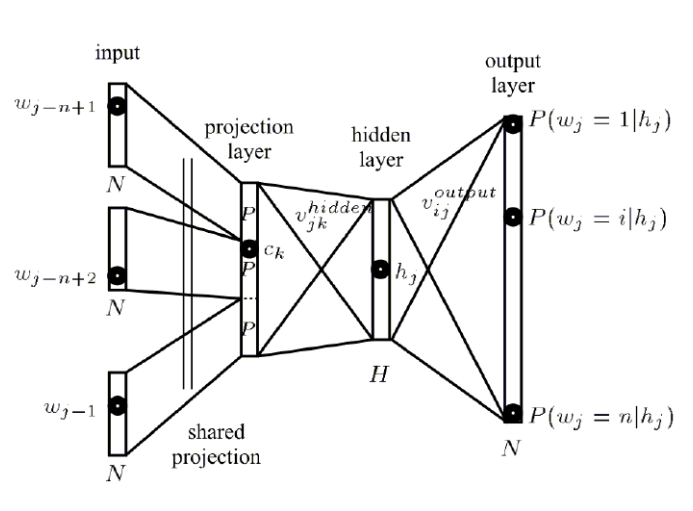
\includegraphics[height=65mm,  width=100mm]{figures/4_languagemodelnn.png}
		\caption[Word2Vec Neural Network Model]{Word2Vec Neural Network Language Model}
			\label{languagemodelnn}
\end{figure}


Word2Vec focuses on distributed representations learned by neural networks~\autoref{languagemodelnn}.  The N-previous words are encoded using 1-of-V hot-vector coding. The words are then projected by a linear operation on the projection layer. Softmax function is used at the output layer to ensure that 0 < = p < = 1. All models are trained and weights are learned using stochastic gradient descent and back propagation. For all models, the training complexity is proportional to:
\begin{center}
 O = E x T x Q,
 \end{center} 
Where, E: \# of Training epochs; T = \# Words in Training Set; Q = Defined further for each model architecture. 

\begin{figure}[ht!]
	\centering
		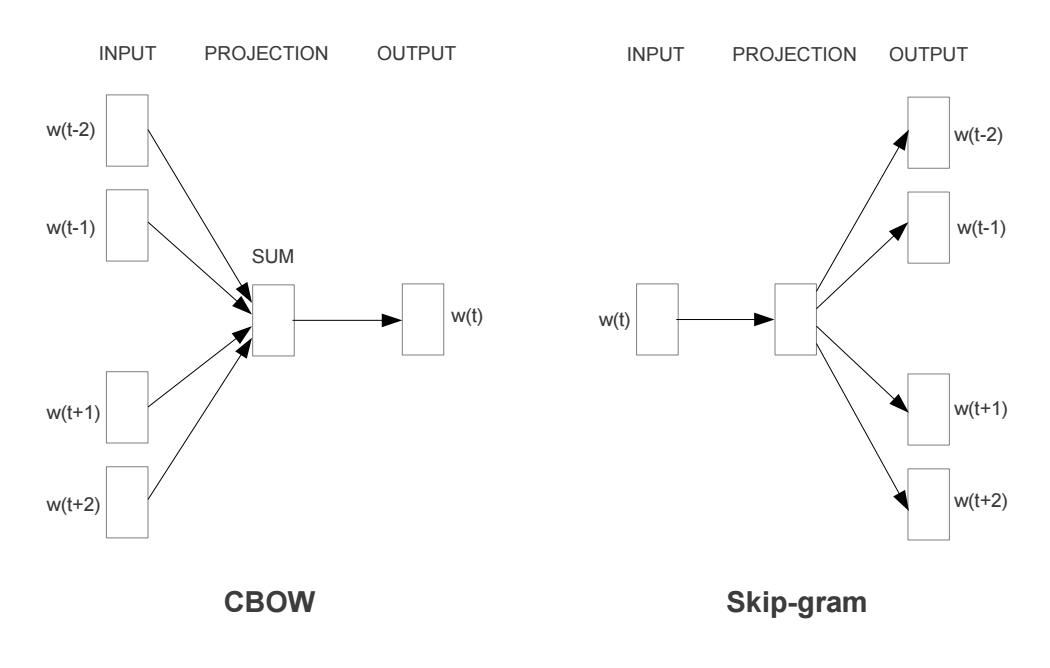
\includegraphics[height=65mm,  width=100mm]{figures/4_w2v.png}
		\caption[Word2Vec Model Architectures]{Word2Vec Model Architectures: CBOW and Skip-Gram}
			\label{w2vmodelarch}
\end{figure}

\textbf{CBOW}: Predicts the current word based on the context.
\begin{itemize}
\item Similar to feed-forward neural network language model, where the non linear hidden layer is removed and projection layer is shared for all words (not just the projection matrix); thus all words are projected into the same position (their vectors are averaged).
\item Best performance, by building the log linear classifier with four future and four history words as input, where training criteria is to correctly classify the current (middle) word.
\end{itemize}
\textbf{SKIP}: Tries to maximize classification of word based on another word in the same sentence.
\begin{itemize}
\item We use each current word as input to a log linear classifier with continuous projection layer and predicts words within a certain range before and after current word.
\end{itemize}

Example: The analogy “\textbf{king is to queen as man is to woman}” should be encoded in the vector space by the vector equation: king - queen = man - woman
\newline

Among the two, the \textbf{Skip-Gram model seems to perform better} with respect to CBOW model on the Word-analogy task (see example above) for both syntactic and semantic categories.

Mikolov et. al  discuss the skip gram model separately in another work ~\parencite{mikolov2}. The training objective for the skip gram model is to find the word representations that are useful for predicting the surounding words in a sentence or a document. More formally, given a sequence of training words ${w}_{1}, {w}_{2}, {w}_{3}, . . . , {w}_{T}$ , the objective of the Skip-gram model is to maximize the average log probability:

\begin{equation}
\frac{1}{T} \sum_{t=1}^{T} \sum_{-c \leq j  \leq c, j \neq 0} log p({w}_{t+j} | {w}_{t})
\end{equation}


where \textbf{c} is the size of the training context (which can be a function of the center word wt). Larger \textbf{c} results in more training examples and thus can lead to a higher accuracy, at the expense of the training time. The basic Skip-gram formulation defines $p({w}_{t+j} | {w}_{t})$ using the softmax function:
\begin{equation}
p({w}_{O}|{w}_{I}) = \frac{exp({{v'}_{wO}}^{T} {v}_{wI} )}{ \sum_{w=1}^{W} exp({{v'}_{w}}^{T} {v}_{wI} ) }
\end{equation}

where ${v}_{w}$ and ${v'}_{w}$ are the “input” and “output” vector representations of w, and W is the number of words in the vocabulary. 
\newline

\textbf{Hierarchical Softmax} ~\parencite{morbengio} is computationally more efficient than the traditional softmax. It uses a binary tree representation of the output layer with the W words as its leaves and for each node explicitly represents the relative probabilities of its child nodes. These define a random walk that assigns probabilities to words. The key advantage here is instead of evaluating W output nodes in the neural network to obtain the probability distribution, only about log(W) nodes are required to be evaluated. More precisely, each word w can be reached by an appropriate path from the root of the tree. Let n(w, j) be the j-th node on the path from the root to w, and let L(w) be the length of this path, so n(w, 1) = root and n(w, L(w)) = w. In addition, for any inner node n, let ch(n) be an arbitrary fixed child of n and let [[x]] be 1 if x is true and -1 otherwise. Then the hierarchical softmax defines $p({w}_{O}|{w}_{I})$ as follows:

\begin{equation}
p({w}|{w}_{I}) =  \prod_{j=1}^{L(w)-1}  \sigma  \big( [ n (w, j + 1) = ch (n(w,j))]. {{v'}_{n(w,j)}}^{T} {v}_{wI} \big)
\end{equation}

Where, $\sigma(x) = 1/ (1 + exp(-x)).$
\newline

The work also introduces negative sampling. Its a simplified form of Noise Contrastive Estimation (NCE), which was introduced by Gutmann et al. ~\parencite{gutmann}. This simplification can be done as long as the vector representations retain their quality. Negative Sampling is defined by the objective function:

\begin{equation}
log  \sigma ({{v'}_{{w}_{O}}}^{T} {v}_{{w}_{I}}) +  \sum_{i=1}^{k} {E}_{{w}_{i}  \sim {P}_{n}(w)} [log \sigma ({{-v'}_{{w}_{i}}}^{T} {v}_{{w}_{I}})]
\end{equation}

which is used to replace every $log P({w}_{O}| {w}_{I})$ term in the skip-gram objective. Thus the task is to distinguish the target word ${w}_{O}$ from draws from the noise distribution ${P}_{n}(w)$ using logistic regression, where there are k negative samples for each data sample. After experimental investigations, the unigram distribution $U{(w)}^{3/4}/Z$ outperformed other uniform and unigram distributions.
\newline

Moreover, to counter the imbalance between the rare and frequent words, a simple \textbf{subsampling approach} was used, where each word ${w}_{i}$ in the training set is discarded with probability computed by the formula:

\begin{equation}
P{w}_{i} = 1 -  \sqrt{\frac{t}{f({w}_{i})}}
\end{equation}

where, $f({w}_{i})$ is the frequency of word ${w}_{i}$ and \textbf{ t } is the threshold which is ${10}^{-5}$. The method, aggressively subsamples words whose frequency is greater than \textbf{ t} while preserving the ranking of the frequencies. 

\section{GloVe}
Pennington et al.~\parencite{glove} introduced GloVe or \textbf{Global Vectors for Word Representations}, a global bi-linear regression model that combines the advantages of the two major model families in the literature: global matrix factorization and local context window methods. The model efficiently leverages statistical information by training only on the nonzero elements in a word-word co-occurrence matrix, rather than on the entire sparse matrix or on individual context windows in a large corpus. This study was at large developed to understand why there exists linguistic similarity properties in word embeddings.

Let the matrix of word-word co-occurrence counts be denoted by X, whose entries  ${X}_{ij}$ tabulate the number of times word j occurs in the context of word i. Let  ${X}_{i}$ = $\sum_{k} {X}_{ik}$ be the number of times any word appears in the context of word i. Finally, let ${P}_{ij}$ = $P(j | i)$ = ${X}_{ij}/{X}_{i}$ be the probability that word j appear in the context of word i.

\begin{figure}[ht!]
	\centering
		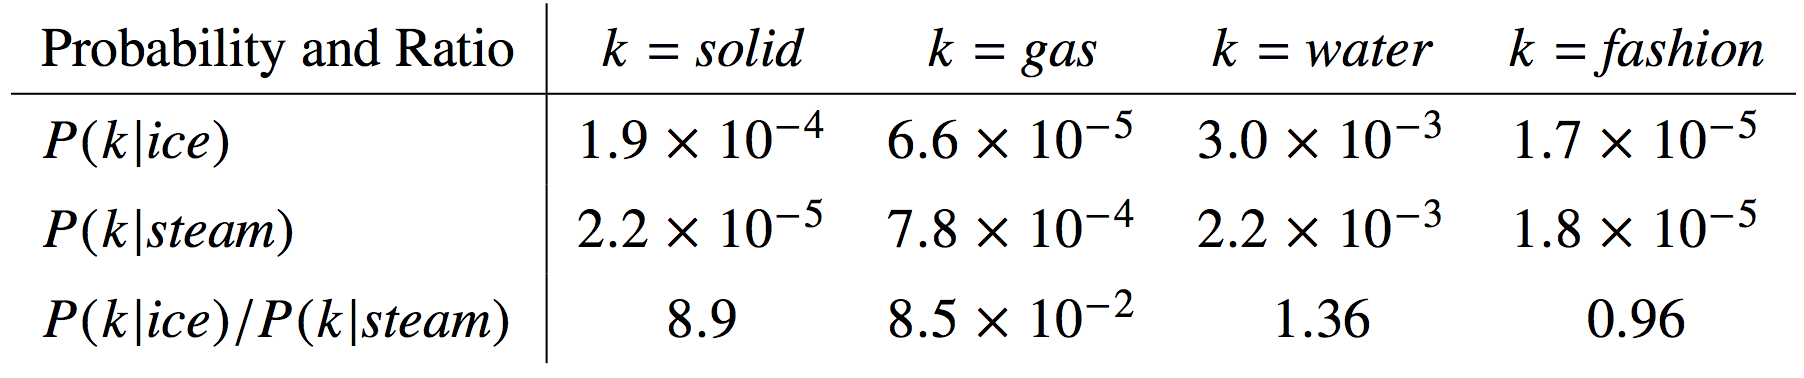
\includegraphics[height=20mm,  width=95mm]{figures/4_glovetable.png}
		\caption[Co-occurrence probabilities for target words]{Co-occurrence probabilities for target words ice and steam with selected context words f}
			\label{glovetable}
\end{figure}

Now considering two words i = ice and j = steam, The relationship of these words ~\autoref{glovetable} can be examined by studying the ratio of their co-occurrence probabilities with various probe words, k. For words k related to ice but not steam, say k = solid, we expect the ratio ${P}_{ik} /{P}_{jk}$ will be large. Similarly, for words k related to steam but not ice, say k = gas, the ratio should be small. For words k like water or fashion, that are either related to both ice and steam, or to neither, the ratio should be close to one. As compared to raw probabilities, the ratio is better able to distinguish relevant words (solid and gas) from irrelevant words (water and fashion) and it is also better able to discriminate between the two relevant words.

As the ratio ${P}_{ik} /{P}_{jk}$ depends on three words i, j and k, the most general model takes the form:

\begin{equation} \label{eq:glove1}
F({w}_{i},{w}_{j},{\tilde{w}}_{k}) = \frac{{P}_{ik}}{{P}_{jk}}
\end{equation}

where, \textit{w} are word vectors and $\tilde{w}$ are context word vectors. F can depend on a number of parameters and the RHS is inferred from the corpus. We wold like F to encode information present in the ration of probabilities, we can achieve this by applying vector differences to ~\autoref{eq:glove1}. 

\begin{equation} \label{eq:glove2}
F({w}_{i} - {w}_{j},{\tilde{w}}_{k}) = \frac{{P}_{ik}}{{P}_{jk}}
\end{equation}

In ~\autoref{eq:glove2} the parameters of F are all vectors whereas the RHS is scalar. Thus, we convert the LHS to scalar by taking a dot product. This also prevents F to mix up vector dimensions undesirably.

\begin{equation} \label{eq:glove3}
F({({w}_{i} - {w}_{j})}^{T}{\tilde{w}}_{k}) = \frac{{P}_{ik}}{{P}_{jk}}
\end{equation}

Note that, for word-word co-occurrence matrices, the distinction between a word and a context word is arbitrary and e can exchange the two roles.  This can be performed on  ~\autoref{eq:glove3} in two steps. First, we require that F be a homomorphism
between the groups (R,+) and (${R}_{>0}$, x), i.e., 

\begin{equation} \label{eq:glove4}
F({{w}_{i} - {w}_{j}}^{T},{\tilde{w}}_{k}) = \frac{F({{w}_{i}}^{T} {\tilde{w}}_{k})}{F({{w}_{j}}^{T} {\tilde{w}}_{k})}
\end{equation}

which by ~\autoref{eq:glove3} is solved by:

\begin{equation} \label{eq:glove5}
F({{w}_{i}}^{T} {\tilde{w}}_{k}) = {P}_{ik} = \frac {{X}_{ik}}{{X}_{i}}
\end{equation}

The solution to ~\autoref{eq:glove4} is F = exp,

\begin{equation} \label{eq:glove6}
{{w}_{i}}^{T} {\tilde{w}}_{k}  = log( {P}_{ik} ) = log({X}_{ik} ) - log({X}_{i}) .
\end{equation}

In ~\autoref{eq:glove6}, the term  $log({X}_{i})$ is independent of  \textbf{k} so it can be absorbed into a bias ${b}_{i}$ for  ${w}_{i}$. Finally, adding an additional bias  ${\tilde{b}}_{k}$ for ${\tilde{w}}_{k}$ restores the symmetry,

\begin{equation} \label{eq:glove7}
{{w}_{i}}^{T} {\tilde{w}}_{k} +  {b}_{i} +  {\tilde{b}}_{k} = log({X}_{ik}).
\end{equation}

There are two problems with ~\autoref{eq:glove7}, first, when argument is zero for logarithm, it diverges. This can be overcome by substitution of  $log({X}_{ik})  \rightarrow  log(1 + {X}_{ik})$. Another drawback is that the model weighs all occurrences equally even for those which happen rarely or never. 

Finally we model ~\autoref{eq:glove7} as new weighted least squares regression model that addresses these problems. A weighting function $f(log({X}_{ij})$ is introduced into the
cost function giving us:

\begin{equation} \label{eq:glove8}
 J =  \sum_{i,j=1}^{V}  f \big({X}_{ij}\big)  {\big({{w}_{i}}^{T} {\tilde{w}}_{k} +  {b}_{i} +  {\tilde{b}}_{k} - log({X}_{ik})\big)}^{2}.
\end{equation}

where V is size of Vocabulary. The choice of function f was generalized as follows:

\begin{equation} \label{eq:glove9}
f (x) =\begin{cases}{(x/{x}_{max})}^{\alpha} & x < {x}_{max}\\1 & otherwise\end{cases} 
\end{equation}

\begin{figure}[ht!]
	\centering
		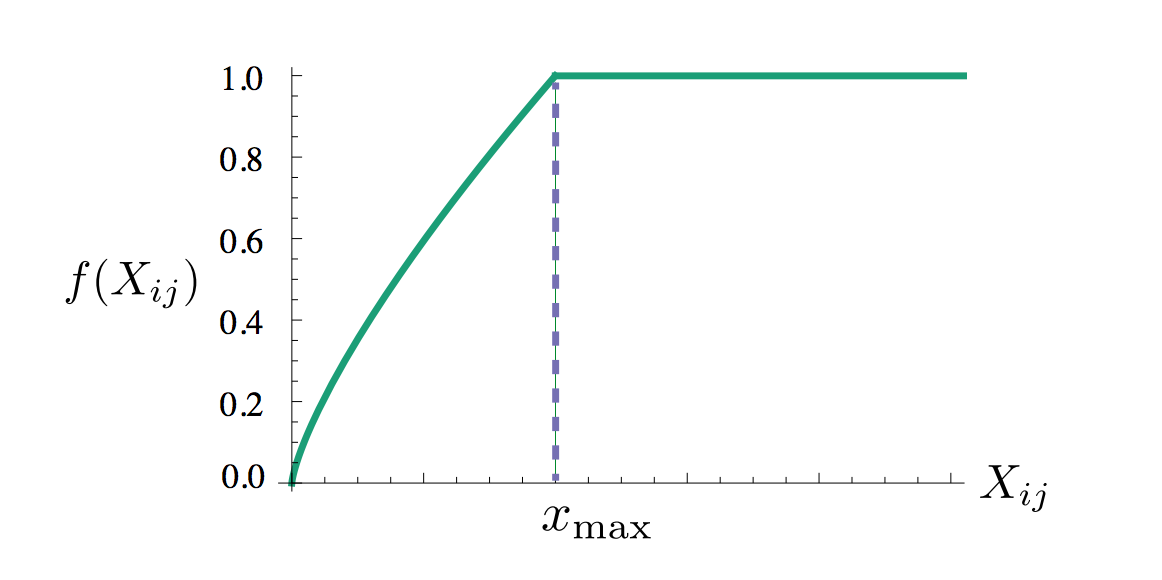
\includegraphics[height=35mm,  width=55mm]{figures/4_weightfunction.png}
		\caption[Glove Weight Function]{GloVe Weight Function f with $\alpha$ =3/4}
			\label{glovefunction}
\end{figure}


The value for ${x}_{max}$ was fixed at 100 and value of $\alpha = 3/4$  ~\autoref{glovefunction} provided modest improvement over $\alpha = 1$ after experimental evaluation. Thus the, ~\autoref{eq:glove8}  is the final GloVe model. Interestingly, The GloVe model beat the Word2Vec model on the standard analogy task on both the syntactic and semantic categories. 
  
\section{Polyglot}

Rami Al-Rofou et. al, ~\parencite{polyglot:2013:ACL-CoNLL} trained word embeddings for more than 100 languages using their corresponding Wikipedias and evaluated them against a standard Part of Speech (POS) tagging task. To construct the objective function for the neural network, a given sequence of words $S  = [{w}_{i-n} \cdots {w}_{i}  \cdots {w}_{i+n}]$ observed in the corpus T,  another corrupted sequence S'  is constructed by replacing the word in the middle ${w}_{i}$ with a word ${w}_{j}$ chosen at random. The neural network represents a function score that scores each phrase, the model is penalized through the hinge loss function J(T) as shown in ~\autoref{eq:polyglot1} 
\begin{equation} \label{eq:polyglot1}
J(T) = \frac{1}{|T|}  \sum_{i  \in T} {|1 - score(S') + score(S)|}_{+} 
\end{equation}

First, each word is mapped through a vocabulary dictionary, size |V| to an index that is used to index a shared matrix C with the size |V| $\times$ M ~\autoref{polyglotnn}. Here, M is the size of the vector representing the word. 

These vectors are then concatenated into one vector called projection layer P with size (2n + 1) $\times$ M. The projection layer plays the role of an input to a hidden layer with size |H|, the activations A of which are calculated according to equation 3, where ${W}_{1}$, ${b}_{1}$ are the weights and bias of the hidden layer. 

\begin{equation} \label{eq:polyglot2}
A = tanh({W}_{1}P +  {b}_{1}) 
\end{equation}

To calculate the phrase score, a linear combination of the hidden layer activations A is computed using ${W}_{2}$ and ${b}_{2}$ .

\begin{equation} \label{eq:polyglot3}
score(P) = {W}_{2}A + {b}_{2} 
\end{equation}

Therefore, the five parameters that have to be learned are ${W}_{1}$ , ${b}_{1}$, ${W}_{2}$, ${b}_{2}$ and C.

\begin{figure}[ht!]
	\centering
		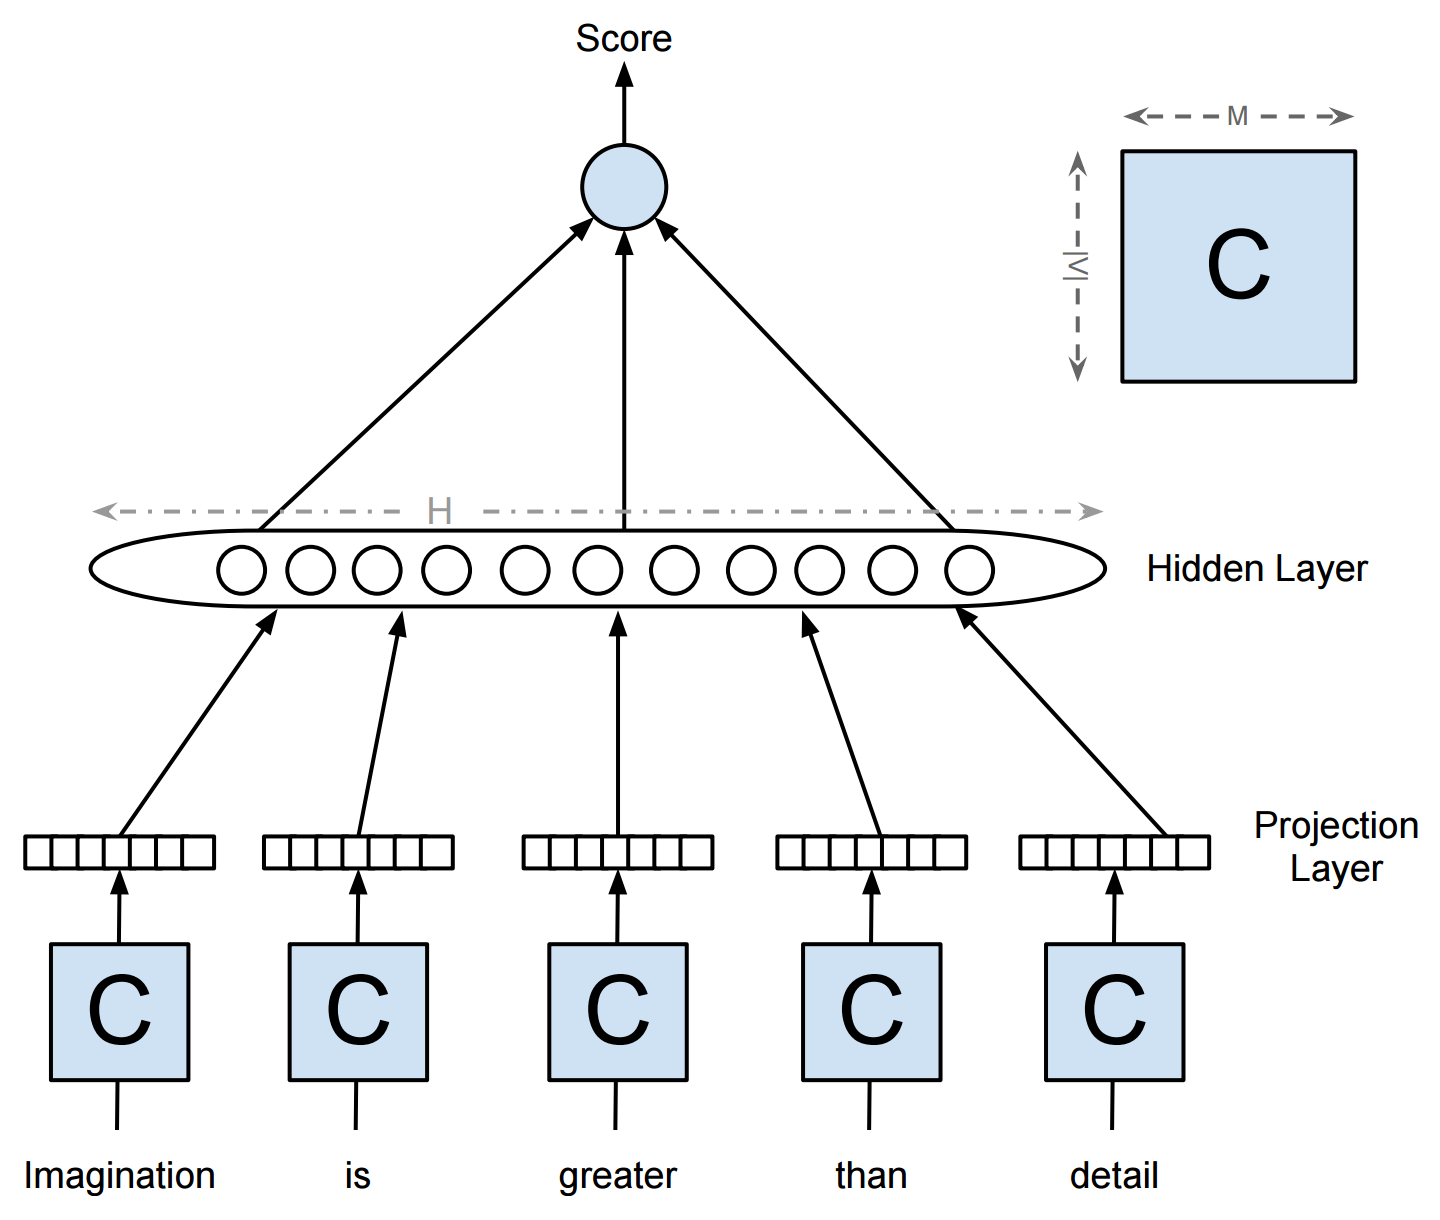
\includegraphics[height=60mm,  width=70mm]{figures/4_polyglotnn.png}
		\caption[Polyglot Neural Network Architecture]{Polyglot Neural Network Architecture}
			\label{polyglotnn}
\end{figure}

\section{Paragraph Vectors}

Quoc Le and Thomas Mikolov~\parencite{paragraphvectors} introduced Paragraph Vectors, an unsupervised algorithm that learns fixed length fixed representations from variable lengths texts like sentences, paragraphs and documents. The algorithm \textbf{represents an entire document as a dense vector}, which is trained to predict words in the document.  The inspiration for paragraph vectors are the vectors, which are asked to predict the next word in the sequence. And even though these vectors are randomly initialized, they can contribute to the semantics and capture semantic similarity as an indirect side-effect of this prediction task. What makes paragraph vectors different is that they too contribute to prediction task, but the context is not words but paragraphs. They build upon the earlier work done by Mikolov et al. ~\parencite{mikolov1}~\parencite{mikolov2} and use the same fundamental objective function and additionally now uses both words and paragraph vectors as context. 

\begin{figure}[ht!]
	\centering
		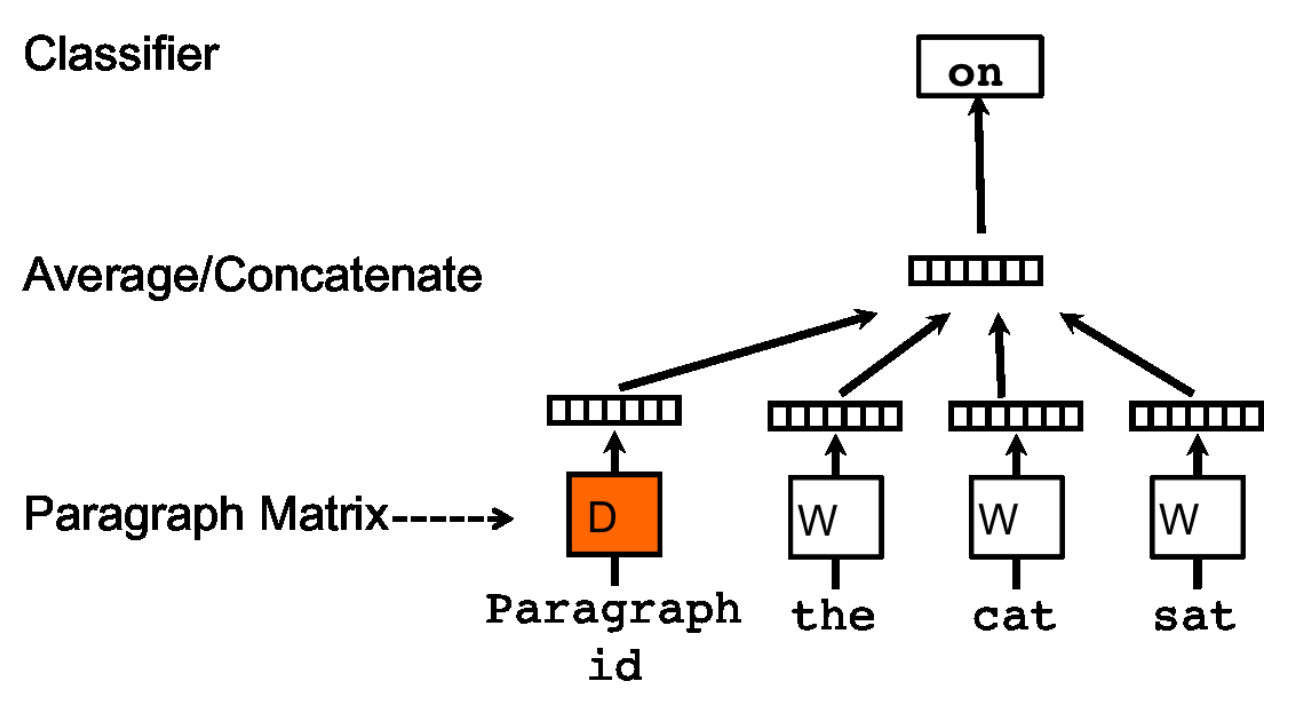
\includegraphics[height=55mm,  width=90mm]{figures/4_paragraphvectors.png}
		\caption[Learning Paragraph Vectors]{Framework for Learning Paragraph Vectors}
			\label{paragraphvectors}
\end{figure}

The framework for learning paragraph vectors can be seen in ~\autoref{paragraphvectors}. every paragraph is mapped to a unique vector D along with the words which are mapped to a unique word vector W. The paragraph vectors and the word vectors are concatenated or averaged to predict the next word in the sentence. When learning paragraph vectors, both D and W are used. The paragraph token can be seen as just another word. This acts as a memory which preserves the topic of the paragraph. It's for this reason, paragraph vector model is also known as Distributed Memory Model of Paragraph Vectors (PV-DM). The context window is fixed and sampled using a sliding window across paragraphs. The paragraph vector is shared across all the contexts generate across same paragraph, whereas the word vectors are shared across all the paragraphs in the document. Both vectors are trained using stochastic gradient descent and the gradient is obtained using back-propagation. At prediction time, we perform an inference step which computes the paragraph vector for a new paragraph  which is again obtained using stochastic gradient descent, but there the parameters for the model softmax and word vectors W are fixed.  

\section{Interesting properties of Word Vectors}
Word Vectors have a very interesting property, when these word vectors are projected in high dimensional space, the semantically closer words are found to be similar to each other. This was highlighted first in Word2Vec and then later in GloVe. Few examples are shown below visualize them on a 2D plane by using PCA dimensionality reduction ~\autoref{word2vec:countriescapitals} and t-SNE  ~\autoref{glove:gender}.   

\begin{figure}[ht!]
	\centering
		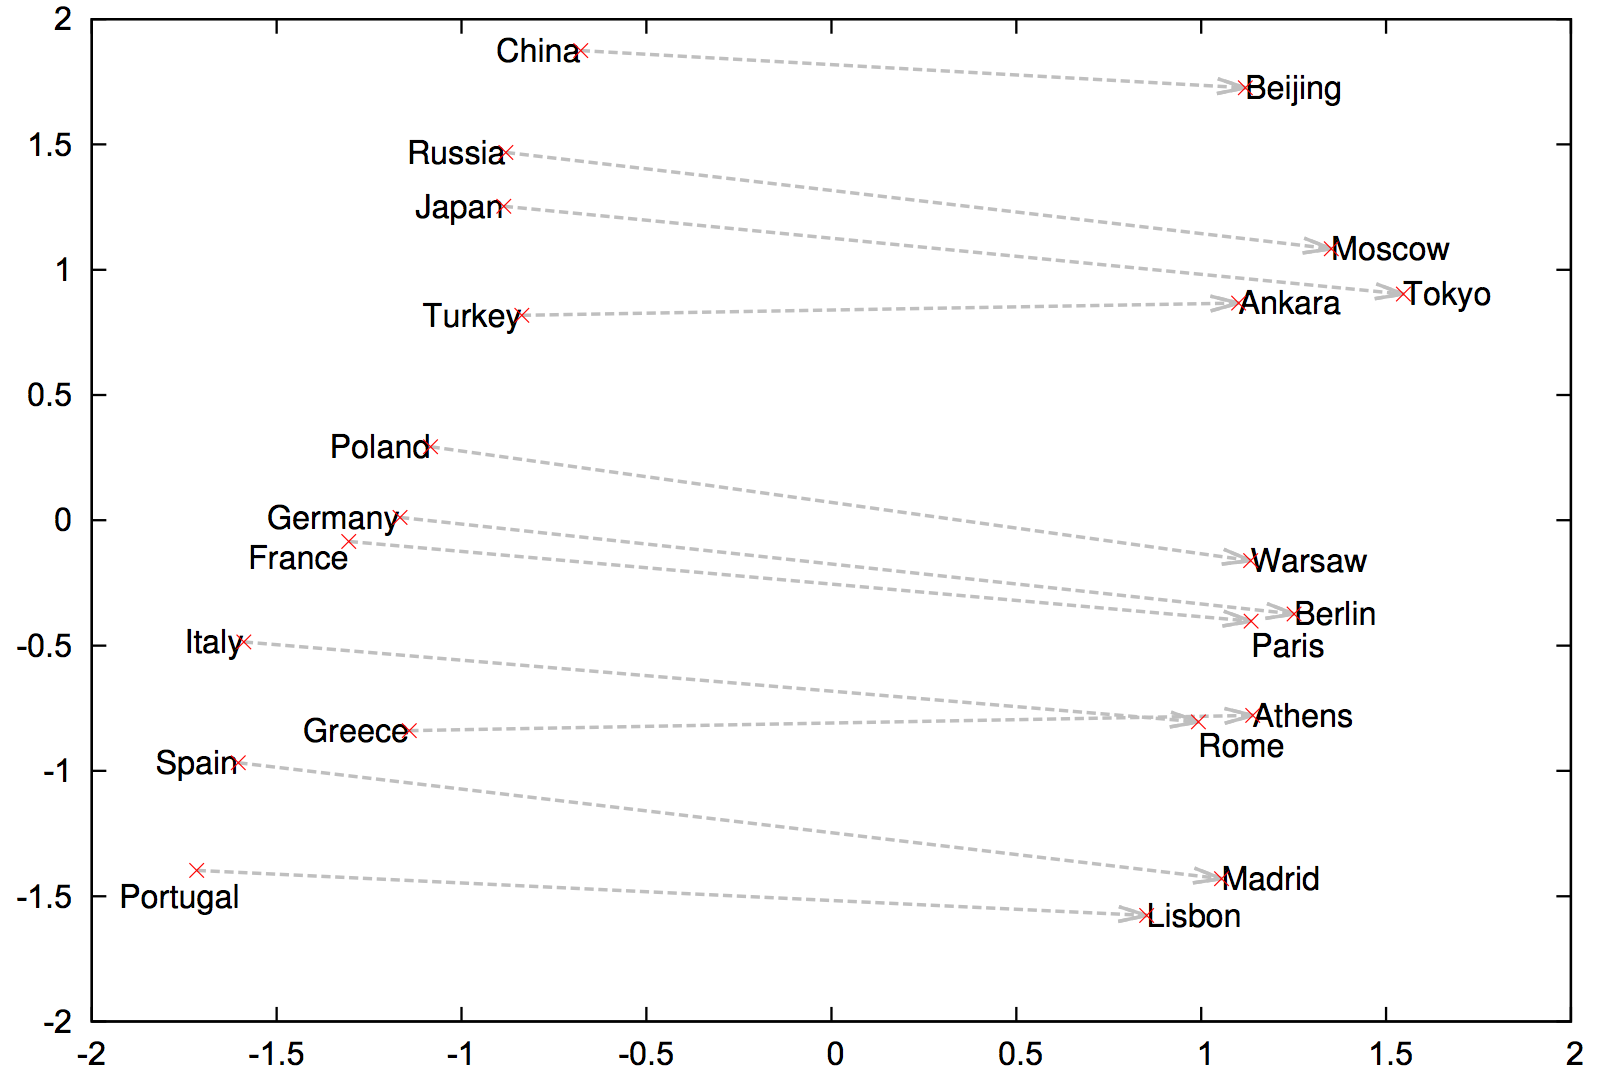
\includegraphics[height=55mm,  width=90mm]{figures/4_countriescities.png}
		\caption[Word2Vec - Countries and Capitals]{Word2Vec - Countries and Capitals Relationship~\parencite{mikolov2}}
			\label{word2vec:countriescapitals}
\end{figure}

\begin{figure}[ht!]
	\centering
		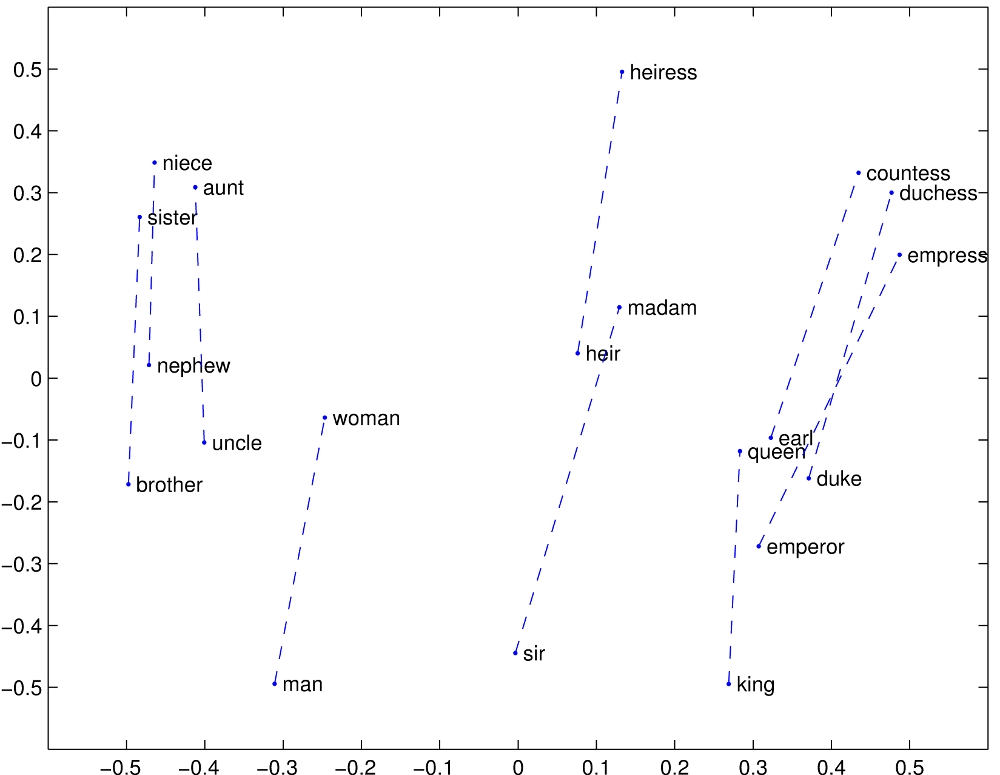
\includegraphics[height=55mm,  width=90mm]{figures/4_manwoman.jpg}
		\caption[GloVe - Gender]{GloVe - Gender Relationship~\parencite{glove}}
			\label{glove:gender}
\end{figure}

A direct result of these are the analogy relations based on difference vectors. For Example:
\textit{v("king") - v("queen") = v("man") - v("woman")}